\documentclass[a4paper]{article}
\usepackage{graphicx, indentfirst, algorithm, algorithmic, float, hyperref}
\graphicspath{{img/}}

\title{Cloud Computing Paper Reading Report}
\author{Jianzhong LI 13354146, Tong XU 13354146, Zhengyuan WEI 13354146}

\begin{document}
  \maketitle
  \section{ImageNet Classification with Deep Convolutional Neural Networks}
      \subsection{Basic Idea}
      
          In this paper, Alex et al. trained a large, deep convolutional neural network to classify the 1.2 million high-resolution images in the ImageNet LSVRC-2010 contest into the 1000 different class. As depicted in Figure 1, the net contains eight layers with weights, the first five are convolutional and remaining three are fully-connected. The output of the last fully-connected layer is fed to a 1000-way softmax which produces a distribution over the 1000 class labels.
      
      \begin{figure}[h]
      \centering
      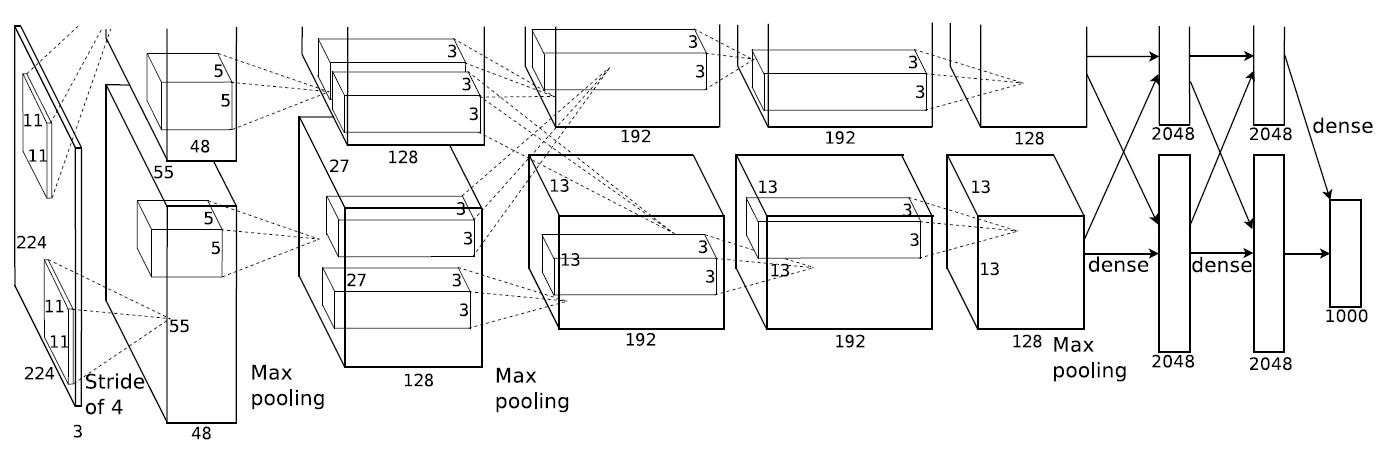
\includegraphics[width=0.7\linewidth]{screenshot002}
      \caption{An illustration of the architecture of CNN, explicitly showing the delineation of responsibilities between the two GPUs.}
      \label{fig:screenshot002}
      \end{figure}

      
      \subsection{Motivation}
      
      \begin{enumerate}
          \item As the traditional approaches of object recognition arrives its bottleneck, using deep learning technical to solve this problem is more and more popular, but for large dataset like ImageNet, which consists of over 15 million labeled high-resolution images in over 22,000 categories, a poor designed convolutional Neural will be easy to be \textbf{over fitting}.
          \item For a convolutional neural network, it needs millions of parameters and lots of memory. If we train the neural network just on a single GPU, it will crash because it can't hold that humongous convolutional neural network.
      \end{enumerate}
      
      \subsection{Contribution}
      
      \begin{enumerate}
          \item Alex et at. proposed to use ReLU Nonlinearity as the neuron's output function, which is times faster than tanh(x) and sigmoid function.
          \begin{figure}[h]
          \centering
          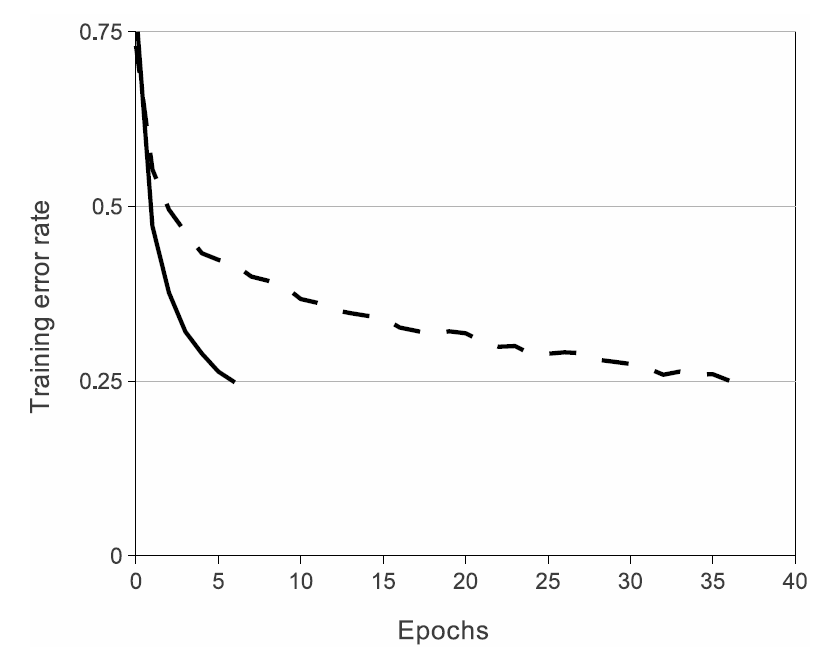
\includegraphics[width=0.7\linewidth]{screenshot001}
          \caption{A four-layer convolutional neural network with ReLUs\textbf{(solid line)} reaches a 25\% training error rate on CIFAR-10 six times faster than an equivalent network with tanh neurons\textbf{(dashed line)}}
          \label{fig:screenshot001}
          \end{figure}

          \item A single GTX 580 GPU has only 3GB of memory, which limits the maximum size of the network that can be trained on it. Therefore Alex et al. proposed to train the net across two GPUs. It allows us to train the big CNNs.
      \end{enumerate}
      
      \subsection{Comments}
      In our project, we use convolutional neural network to classify the picture. This paper gives us a very good CNN architecture. It can speed up the train phase and save computing resources. We use \href{http://caffe.berkeleyvision.org/}{Caffe} to build this model, which is a excellent framework for deep learning.

  \section{Fast R-CNN}
    
      \subsection{Basic Idea}
          Rbg et al. proposed Fast R-CNN, a clean and fast framework for object detection. Compared to traditional R-CNN, and its accelerated version SPPnet, Fast R-CNN trains network using a multi-task loss in a single training stage. The Fast R-CNN architecture is as follows
          \begin{figure}[h]
          \centering
          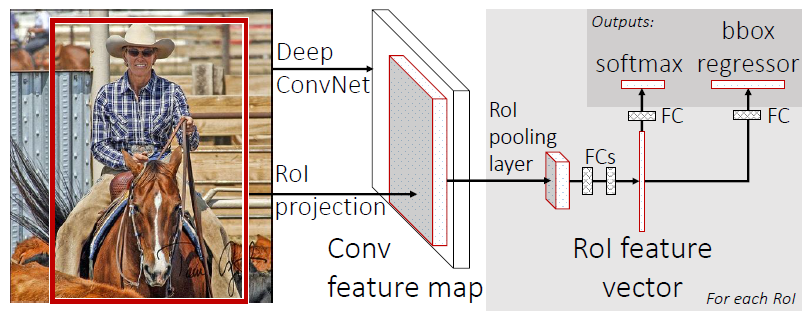
\includegraphics[width=0.7\linewidth]{screenshot003}
          \caption{Fast R-CNN architecture. An input image and multiple
              regions of interest (RoIs) are input into a fully-convolutional
              network. Each RoI is pooled into a fixed-size feature map and
              then mapped to a feature vector by fully-connected layers (FCs).
              The network has two output vectors per RoI: softmax probabilities
              and per-class bounding-box regression offsets. The architecture is trained end-to-end with a multi-task loss.}
          \label{fig:screenshot003}
          \end{figure}

      \subsection{Motivation}
        R-CNN has excellent object detection accuracy. However, it also has notable drawbacks:
        \begin{enumerate}
          \item Training is a multi-stage pipeline. First fine-tunes a ConvNet for detection using cross-entrogy loss. Then. linear SVMs are fit to ConvNet features computed on warped object proposals. In the third training stage, bounding-box regressors are learned.
          \item Training is expensive in space and time. For SVM and regressor training, features are extracted from each warped object proposal in each image and written to disk. These features require hundreds of gigabytes of storage.
          \item Test time detection is slow. At test-time, features are extracted from each warped object proposal in test time. Detection with VGG16 takes 47s/image.
        \end{enumerate}
      \subsection{Contribution}
        They propose a new training algorithm that fixes the disadvantages of R-CNN and SPPnet, while improving on their speed and accuracy. It has the following advantages:
        \begin{enumerate}
          \item Higher detection quality(mAP) than R-CNN
          \item Training is single-stage, using a multi-task loss
          \item All network layers can be updated during training
          \item No disk storage is required for feature caching
        \end{enumerate}
      \subsection{Comments}
        In our project, we use fast rcnn to detect objects, since it's a clean and fast update to R-CNN and SPPnet. Although sparse object proposal appear to improve detector quality, but it is too costly in time. We want to develop a more accelerate object detection neural network in our further work.  
    
  \section{Selective Search for Object Recognition}
      \subsection{Basic Idea}
        This paper addresses the problem of generating possible object locations for use in object recognition. They introduce Selective Search which combines the strength of both an exhaustive search and segmentation. It can generate a class-independent, data-driven, selective search strategy that generates a small set set of high-quality object locations.
      \subsection{Motivation}
        For a long time, objects were sought to be delineated before their identification. But images are intrinsically hierarchical and a segmentation should be hierarchical, a generic solution for segmentation using a single strategy may not exist at all. 
        \begin{figure}[h]
        \centering
        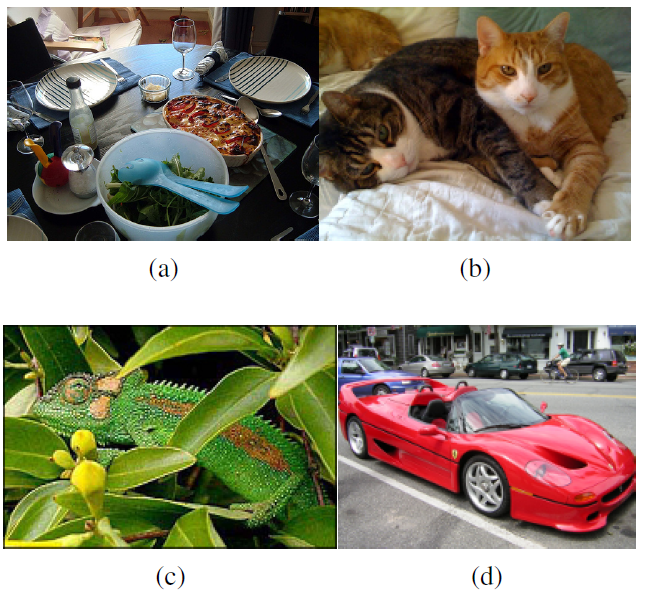
\includegraphics[width=0.7\linewidth]{screenshot004}
        \caption{Images are intrinsically hierarchical:In (a) the salad and spoons are inside the salad bowl, which in turn stands on the table. There is a high variety of reasons that an image region forms an object: In(b) the cats can be distinguished by color and in (c) the chameleon can be distinguished from the surrounding leaves by texture. In (d) the wheels can be part of car because they are enclosed.}
        \label{fig:screenshot004}
        \end{figure}

      \subsection{Contribution}
        This Selective Search algorithm has the advantages as follows:
        \begin{enumerate}
          \item Object can occur at any scale within the image. Furthermore, some objects have less clear boundaries than other objects. Therefore, in selective search all object scales is under consideration.
          \item There is no single optimal strategy to group regions together. Therefore, instead of a single strategy which works well with in most cases, they had a diverse set og strategies to deal with all cases.
          \item This algorithm's goal is to yield a set of possible object locations for use in a practical object recognition framework. Therefore, the computing speed is fast and amazing. 
        \end{enumerate}
      \subsection{Comments}  
        In our project, we download the  selective public code and use it's fast version, which can compute a image in 3s. Note that the whole classification procedure is smoothly complex, we don't supply instance classification service. There we use cloud drive to hold user's photos and do it step by step. Then we store the classification result in the MySQL database, and use PHP to communicate with Android applications. In addition, in future, we will add a photo share feature, which allow users to share interesting photo with others. All tasks above can be done in a middle size virtual machine.    

    \section{Implementation: Mobile Face Identity Authentication System on Android Platforms}
    \subsection{Basic idea}
        The paper proposes a mobile face identify authentication system based on distributed computing. The workflow is as follows:
        \begin{enumerate}
          \item Client(Android phone) capture an image
          \item perform local face detection and crop the face rectangle
          \item Facial image and additional information will be sent to the server.
          \item Haar-like features and regular LBP features are extracted, train the classifier with AdaBoost algorithm
          \item validation result returned.
        \end{enumerate}
    \subsection{Motivation}
      Substitution for exams and course is possible in campus due to the relative loose management in universities. To maintain the school education order, a mobile facial authentication system is urgently need and possible to be built with modern cloud computing, artificial intelligence and mobile computing technology.
    \subsection{Contribution}
      The paper propose an implementation of a mobile facial authentication system. The preprocessing on local client (crop the image with face detection and downgrade to grayscale) is quite inspiring. The validation performance is also good, the cost time of verifying a person is about 2  seconds in average and its accuracy is above 90\%.
    \subsection{Comments}
      Interesting. A function structure diagram is also presented in the paper. Our project also need to deal with images. Some of them are people portrait. However, since real time identification is not required, we don’t have to perform any preprocessing. But the architecture of the system proposed in the paper is inspiring.

  \section{Bifocals: Analyzing \texttt{WebView} Vulnerabilities in Android Applications}
    \subsection{Basic idea}
      The paper propose a tool, Bifocals, to detect these vulnerabilities and characterize the prevalence of vulnerable code. Based on the findings, a modification to \texttt{WebView} security policies was suggested that would protect over 60\% of the vulnerable applications with little burden on developers.
    \subsection{Motivation}
      Android \texttt{WebView} has two vulnerabilities: excess authorization, where malicious JavScript can invoke Android application code,  and file-based cross-zone scripting, which exposes a device's file system to an attacker, both of which aren't safe. 
    \subsection{Contribution}
      \begin{itemize}
        \item Build a tool to identify vulnerable WebViews
        \item Meausre the prevalence and impact of vulnerable WebViews
        \item Suggest and evaluate solutions to migrate these vulnerabilities.
      \end{itemize}
    \subsection{Comments}
      \texttt{WebView} is an important component in the Android framework. With \texttt{WebView} we can make use of those awesome tools of great benefits. There are people trying to accomplish crazy things in pure JavaScript, and they invented \texttt{three.js, React.js, Node.js...} etc. Actually there are \texttt{RxAndroid} and \texttt{Electron}, which help people make Android and desktop application in the way of web app. While benefiting from their goodness, the vulnerabilities of Android \texttt{WebView} should draw more attentions.

  \section{A GUI Crawling-based technique for Android Mobile Application Testing}
    \subsection{Basic Idea}

      The papre addressed the problem of automatic testing of mobile applications developed for Android platform, and presents a technique for rapid crash testing and regression testing. The technique is based on a crawler that automatically builds a model of the application GUI and obtains test cases that can be automatically executed.

    \subsection{Motivation} 

      Since testing a mobile device application is not a trivial task due to several factors, the testing activity is neglected or carried out in a superficial way since it is considered too complex, difficult to automate, expensive and time-consuming. In order to obtain higher quality mobile applications, greater attention should be devoted to the testing activity throughout the development process and effective models, methods, techniques and tools for testing should be available for testers. 

    \subsection{Contribution}

      The paper propose a GUI crawling based technique for crash testing and regression testing of Android applications, supported by a tool for producing test cases that can be automatically executed, which make the testing result more reliable while being automatic
    
    \subsection{Comments}
    
      The paper have not considered other types of events that may solicit a mobile application (like external events produced by hardware sensors, chips, network, or other applications running on the same mobile device) and just focused on user events produced through the GUI. But the model is very inspiring. I am interested GUI automatic testing. This paper gives a better understanding of how those framework works.

  \section{FlowDroid: Precise Context, Flow, Field, Object-sensitive and Lifecycle-aware Taint Analysis for Android Apps}
    \subsection{Basic Idea}

      The paper presented F\textsc{LOW}D\textsc{ROID} a novel and highly precise static taint analysis for Android applications. An open test suite, D\textsc{ROID}B\textsc{ENCH} is also proposeed for evaluating the effective ness and accuracy of taint-analysis tools specifically for Android apps. F\textsc{LOW}D\textsc{ROID} succefully finds leaks in a subset of 500 apps from Google Play and about 1,000 malware apps from the VirusShare project.
    \subsection{Motivation}

      While smartphone being a ubiquitous source of private and confidential data, smartphone users are vulnerable tocarelessly programmed apps that leak important data by accident, and malicious apps that exploit their given privileges to copy such data intentionally. Existing static taint-analysis approaches have the potential of detecting such data leaks ahead of time and all approaches for Android use a number of coarse-grain approximations that can yield high numbers of missed leaks and false alarms. A novel and highly precise static taint analysis for Android applications are needed.
    \subsection{Contribution}
      \begin{itemize}
        \item F\textsc{LOW}D\textsc{ROID}, the first fully context, field, object and flowsensitive taint analysis which considers the Android application lifecycle and UI widgets, and which features a novel, particularly precise variant of an on-demand alias analysis;
        \item a full open-source implementation of F\textsc{LOW}D\textsc{ROID}
        \item D\textsc{ROID}B\textsc{ENCH}, a novel, open and comprehensive micro benchmark suite for Android flow analyses
        \item a set of experiments confirming superior precision and recall of F\textsc{LOW}D\textsc{ROID} compared to the commercial tools AppScan Source and Fortify SCA, and
        \item a set of experiments applying FLOWDROID to over 500 apps from Google Play and about 1000 malware apps from the VirusShare project.
      \end{itemize}
    \subsection{Comments}
      At the end of the paper, the authors mentioned that
      \begin{quote}
        We hope that in the future DROIDBENCH will serve as a standard test set for Android taint analyses.
      \end{quote}
      Currently the provided Android test suite mainly focus on non-security related area. Though today various awesome framworks make mobile application development easy, security is an important issue that we can't ignore.

  \section{Instant Messaging Service on Android Smartphones and Personal Computers}

    \subsection{Basic Idea}
      Implement a solution that allows android based smartphone and tablet users to send and receive messages over the intranet via Wi-Fi which requires neither any internet connectivity nor any messaging service from the mobile service providers as shown in the following steps.
      \begin{enumerate}
      \item First of all server program runs on server machine
      \item Then client program runs on android based mobile device and send a request to connect with server
      \item Once the client is successfully connected, the server broadcast the list of all other active users to the client
      \item Client can view the list of all active users and can communicate with them
      \end{enumerate}
      Server creates a separate connection for each client, so one server can serve multiple client.

    \subsection{Motivation}
      The movivation is to allow the smartphone and tablet users to communicate in the intranet without paying any internet data charges.

    \subsection{Contribution}
      This paper presents an idea to develop a service for the intranet users, this service will be deployed on the intranet server of any organization that allows smartphone and tablet users to send and receive messages within an organization at free of cost.

    \subsection{Comments}
      In our project, we need to implement the instant message between android phone and the server. The paper pose a very easy way to implement it. The main idea is the buddy list and contact list as long as the person is online. For our project, it is enough to use to finish out target.
      
  \section{The Interaction Mechanism based on JSON for Android Database Application}

    \subsection{Basic Idea}
      In the Android system, the application and the database server can not interact directly only if use a Web server interaction. It is necessary to use the Web server to complete the operation on the database, such as addition, deletion, alteration and so on. And then exchange data between Android application and Web server, so as to achieve the purpose that Android application operates the database. And in this process, the data format is JSON.
      Just as show here:
      \begin{figure}[h!]
        \centering
        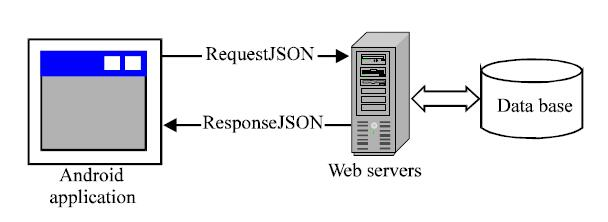
\includegraphics[width=7cm]{android-database-json.jpg}
        \caption{Android application and the database interaction}
        \label{fig-sample}
      \end{figure}

    \subsection{Motivation}
      With the release of a new generation intelligent phone Android and global 3G network into operation, th ecommunications between intelligent phone platform and database server become more and more important. To the constraints of the mobile phone platform memory capacity, the framework of communication mechanism used the light-weight type JSON data format as the transmission medium and used the design patterns of model-view-controller.
      
    \subsection{Contribution}
      By using the MVC development mode and JSON data format, the authors reached the purpose of data interaction between Android application and the database and made a simple optimization.
      
    \subsection{Comments}
      As same as the reading report above, we want instant message and we choose the format of the message is JSON. This paper help us how to use GSON (a package of JSON in Android) to communicate with servers. And this help a lot.
      
  \section{Passwords for both Mobile and Desktop Computers: ObPwd for Firefox and Android}

    \subsection{Basic Idea}
      The obPwd is a existed algorithm to mapping object to a password with ObPwd tool.
      The paper is to study the cross-platform/cross-device implementations. The current implementations use SHA-1 to hash password objects. The hash output is mapped to a base-64 character set, then converted to an alphanumeric password (default 12 characters) by known techniques. Up to the first n = 100000 bytes are used from an object; 160 bytes are required. The final function is the same of we known, pwd = Hash2Text(Hash(URLdomain || fileContent)).

    \subsection{Motivation}
      People wish passwords would go away. But the Internet world continues to have a deep investment in passwords. So this is the motivation the authors want to study passwords. The major goal is to increase attention to the cross-device password authentication problem.
      
    \subsection{Contribution}
      The implementations discussed herein are an illustrative example intended to motivate further discussion and innovation addressing the problem of user-friendly password authentication from alternating computing devices supporting divergent user input capabilities. No doubt, better mechanisms will appear over time. Their chances of deployment success in practice will be much higher if designed from the start keeping in mind cross-device requirements as discussed herein

    \subsection{Comments}
      As same as the reading report above, we want instant message and JSON to return the data. But consider of the secure of the JSON data, data needs to be encipher. This paper show us a method to encipher the same data, and it is usable both in Android and Personal Computer. This means the server can also use the technology to implement the encihption. This help much of our project.



\end{document}